\section{Redes escalables}
\subsection{Redes de Área Locales (LAN)}
\begin{figure}[H]
	\centering
	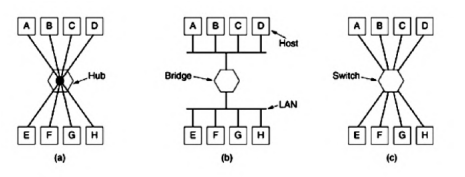
\includegraphics[width=\textwidth
]{images/topologias-red.png}
	\caption[Topologías de Red]{Topologías de Red}
	\label{fig:topologias-red}
\end{figure}
En la figura \label{fig:topologias-red} se pueden ver tres tipos de LAN:
\begin{enumerate}[a)]
  \item En la primera vemos un conjunto de hosts conectados por un \textbf{hub}, esto es: Todos los hosts están conectado
  s entre sí como si los uniese un único cable. El \textbf{hub}, como los \textbf{repetidores} (amplificadores de señal), funcionan a nivel físico permitiendo agregar equipos a una red.
  \item En el segundo, un puente o \textbf{bridge}, separa en dos grupos los hosts de la red creando dos zonas independientes para la detección de colisiones. En este caso los hosts de un grupo podrán emitir sin tener que preocuparse por interferir con los hosts del otro grupo. Un paquete enviado la dirección de \textbf{broadcast}, alcanza a todos los hosts de la LAN.
  
  Puede interconectar, dos tipos de tecnología distintas (por ejemplo, ethernet y wifi). Por esta razón en la capa MAC, se agrega al header del paquete un campo que permite identificar el tipo de red del que viene. Cuando el bridge capta el paquete y se da cuenta que el host está en una red de distinto tipo, cambia el header para que matcheen y lo reenvía a través de la tecnología correspondiente
  \item Por último tenemos un conjunto de host conectados por un \textbf{switch}: Cada host se conecta con una conexión full-duplex al dispositivo, que se encarga de recibir todos los mensajes de un host y redireccionarlo al host correspondiente. En este tipo de redes se elimina la necesidad detectar colisiones y se pasa a necesitar un algoritmo que permita al switch realizar el dispatch de los mensajes de manera correcta.
  
  Tanto el switch como el bridge funciona a nivel capa de enlace. Se encargan de redireccionar los frames enviados a través de una LAN para que lleguen al dispositivo correspondiente.
\end{enumerate}

Agregamos un último dispositivo: El \textbf{router}, para conectar distintas redes a nivel red. Se encargán de buscar el camino que debe seguir para llegar a destino. Cuando una host envía decide enviar un paquete, lo encapsula en un frame que contiene el tipo de protocolo usado. Cuando el paquete llega el router, este se encarga de tomar el frame que le llego, desencapsular el paquete y guardarlo en un frame adecuado para que pueda ser interpretado por los dispositivos de la nueva ren en la que ingresa el frame.

\subsection{Switches}
Son dispositivos que nos permiten interconectar enlaces para formar redes más grandes. 
\red{Repetidores. Puentes. LAN Switches. Conceptos de VLAN y troncales de VLANs (IEEE 802.1Q). Spanning Tree Protocol.
}